\chapter{Studie}
\section{Android}
Android ist, im Gegensatz zu anderen mobilen Betriebssystemen auf dem Markt, eine offene Plattform. Das kommt im Wesentlichen daher, dass Android auf einem open source System, dem Linux Kernel, aufbaut. Durch die freie Verfügbarkeit des Codes, gibt es im Android-Bereich eine große Developer Szene die laufend eigens modifizierte Betriebssysteme (ROMs) und Apps hervorbringt.
Ein so hoher Grad an Offenheit birgt jedoch auch gewisse Sicherheitsrisiken und öffnet Angriffsvektoren. Um diese Gefahren besser zu verstehen sollte man sich eingehend mit der Android Architektur und dem darin enthaltenen Sicherheitskonzept befassen.

\subsection{Architektur}
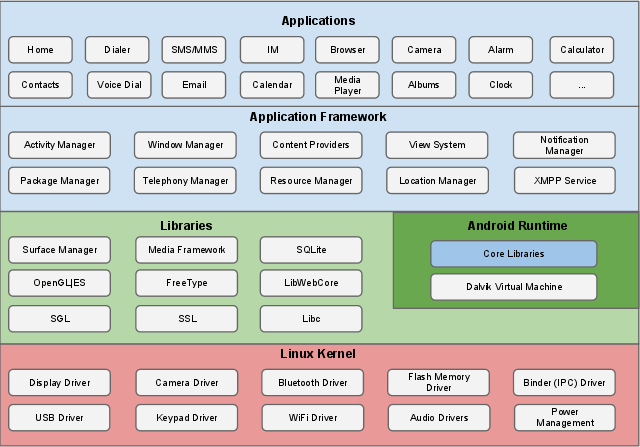
\includegraphics[scale=0.7]{Images/android_stack}
\caption[Android Architektur Schichtenmodell]{Android Architektur }
Wie in Abbildung 1 zu sehen ist, bildet der Linux Kernel die unterste Schicht der Architektur. Auf ihm baut das gesamte Betriebssystem mitsamt aller Sicherheitskonzepte auf. Der Kernel stellt die Brücke zwischen Hard- und Software dar und enthält die Treiber für diverse andere Komponenten eines Smartphones wie beispielsweise Modem, GPS Empfänger, Kamera, etc… \newline
In der darüber liegende Ebene sind die Android Libaries sowie die Runtime, also die „Dalvik Virtual Machine“ zu finden. \newline
Android Apps sind meist in Java Programmiert und werden jeweils in einer eigenen Virtuellen Maschine ausgeführt, der DVM . Diese Systematik ermöglicht das logische parallele, unabhängige Ausführen von verschiedenen Apps mit verschiedenen Benutzerrechten.
Die Libaries steuern und kontrollieren im Wesentlichen die Funktionen des Kernels und sind für die zentralen Funktionalitäten auf niedriger Ebene zuständig.\newline
Die nächst-höhere Ebene bildet das Application Framework. Hier befinden die Grundfunktionen von Android wie zum Beispiel Telefonie, Location Services, Window Manager, Notification Manager, etc… 
Auf dieser Ebene werden Entwicklern äußerst umfangreiche APIs für das Entwickeln von Benutzeranwendungen (Apps) zur Verfügung gestellt. \newline
Die oberste Schicht in der Android-Systemarchitektur sind die Applikationen welche der Benutzer selbst installiert und auf den darunterliegenden Schichten aufbaut.
Dieser gesamte „Stack“ (=Stapel) wird in einem ROM zusammengefasst und auf ein Smartphone installiert. Durch die zuvor erwähnte Offenheit des Systems können so durch Modifizieren eines ROM Paketes stark angepasste Versionen von Android entwickelt und verwendet werden.


\subsection{Security}

\subsection{Probleme}